\documentclass{amsdtx}
\usepackage{graphicx}
\usepackage{amsmath}
\usepackage{amssymb}
\usepackage{float}
\usepackage[dvipsnames]{xcolor}
\usepackage{cancel}
\usepackage{enumitem}
\usepackage[margin=.75in]{geometry}
%\usepackage{pythonhighlight}
\usepackage{hyperref}
\usepackage{url}
\title{\kern-2.4cm\sc ANSYS Composite Analysis for Characterization of the  Project Aurora Fin Can}
\author{\sc M. Nichitiu, C. Casebolt}

\date{\sc MIT Rocket Team, Project Aurora}

\begin{document}
\begin{multicols}{2}
 \maketitle
\begin{center}
	~~~~~~~~~~~~~~~~~~
\includegraphics[scale=0.1]{rtlogo.pdf}
\end{center}
\end{multicols}
~\\
\section{Fin}
We begin with a description of the fin and its analysis. 
\subsection{Fin Structure, Characteristics}
\begin{figure}[H]
\centering

\includegraphics[scale=0.05]{finStruct.pdf}
\caption{Side view of the composition of a fin.}	
\end{figure}
Each fin is composed of a G10 core (thickness of 0.125'') followed by 7 plies of carbon fiber (CF) on each side\footnote{~There is a last layer of CF overwrap over the entire fin can exterior to act as protection and a smooth aerodynamic surface; this is discussed later.}. Each CF ply has a thickness of 0.009''. The total thickness is thus
\begin{align}
	0.125\text{''} + 14(0.009\text{''}) = \bf{0.251\text{\bf ''}}
\end{align}
The CF plies have directionality; we chose to stack the 7 plies in the following orientations:
\begin{table}[H]
\centering
\renewcommand{\arraystretch}{1.4}
\begin{tabular}{r|c|c|c|c|c|c|c}
\bf Ply & 1 & 2 & 3 & 4 & 5 & 6 & 7\\\hline
\bf Orientation & 0$^\circ$ & 0$^\circ$ & 45$^\circ$ & 0$^\circ$ & 45$^\circ$ & 0$^\circ$ & 0$^\circ$
\end{tabular}
\end{table}
\begin{figure}[H]
\centering
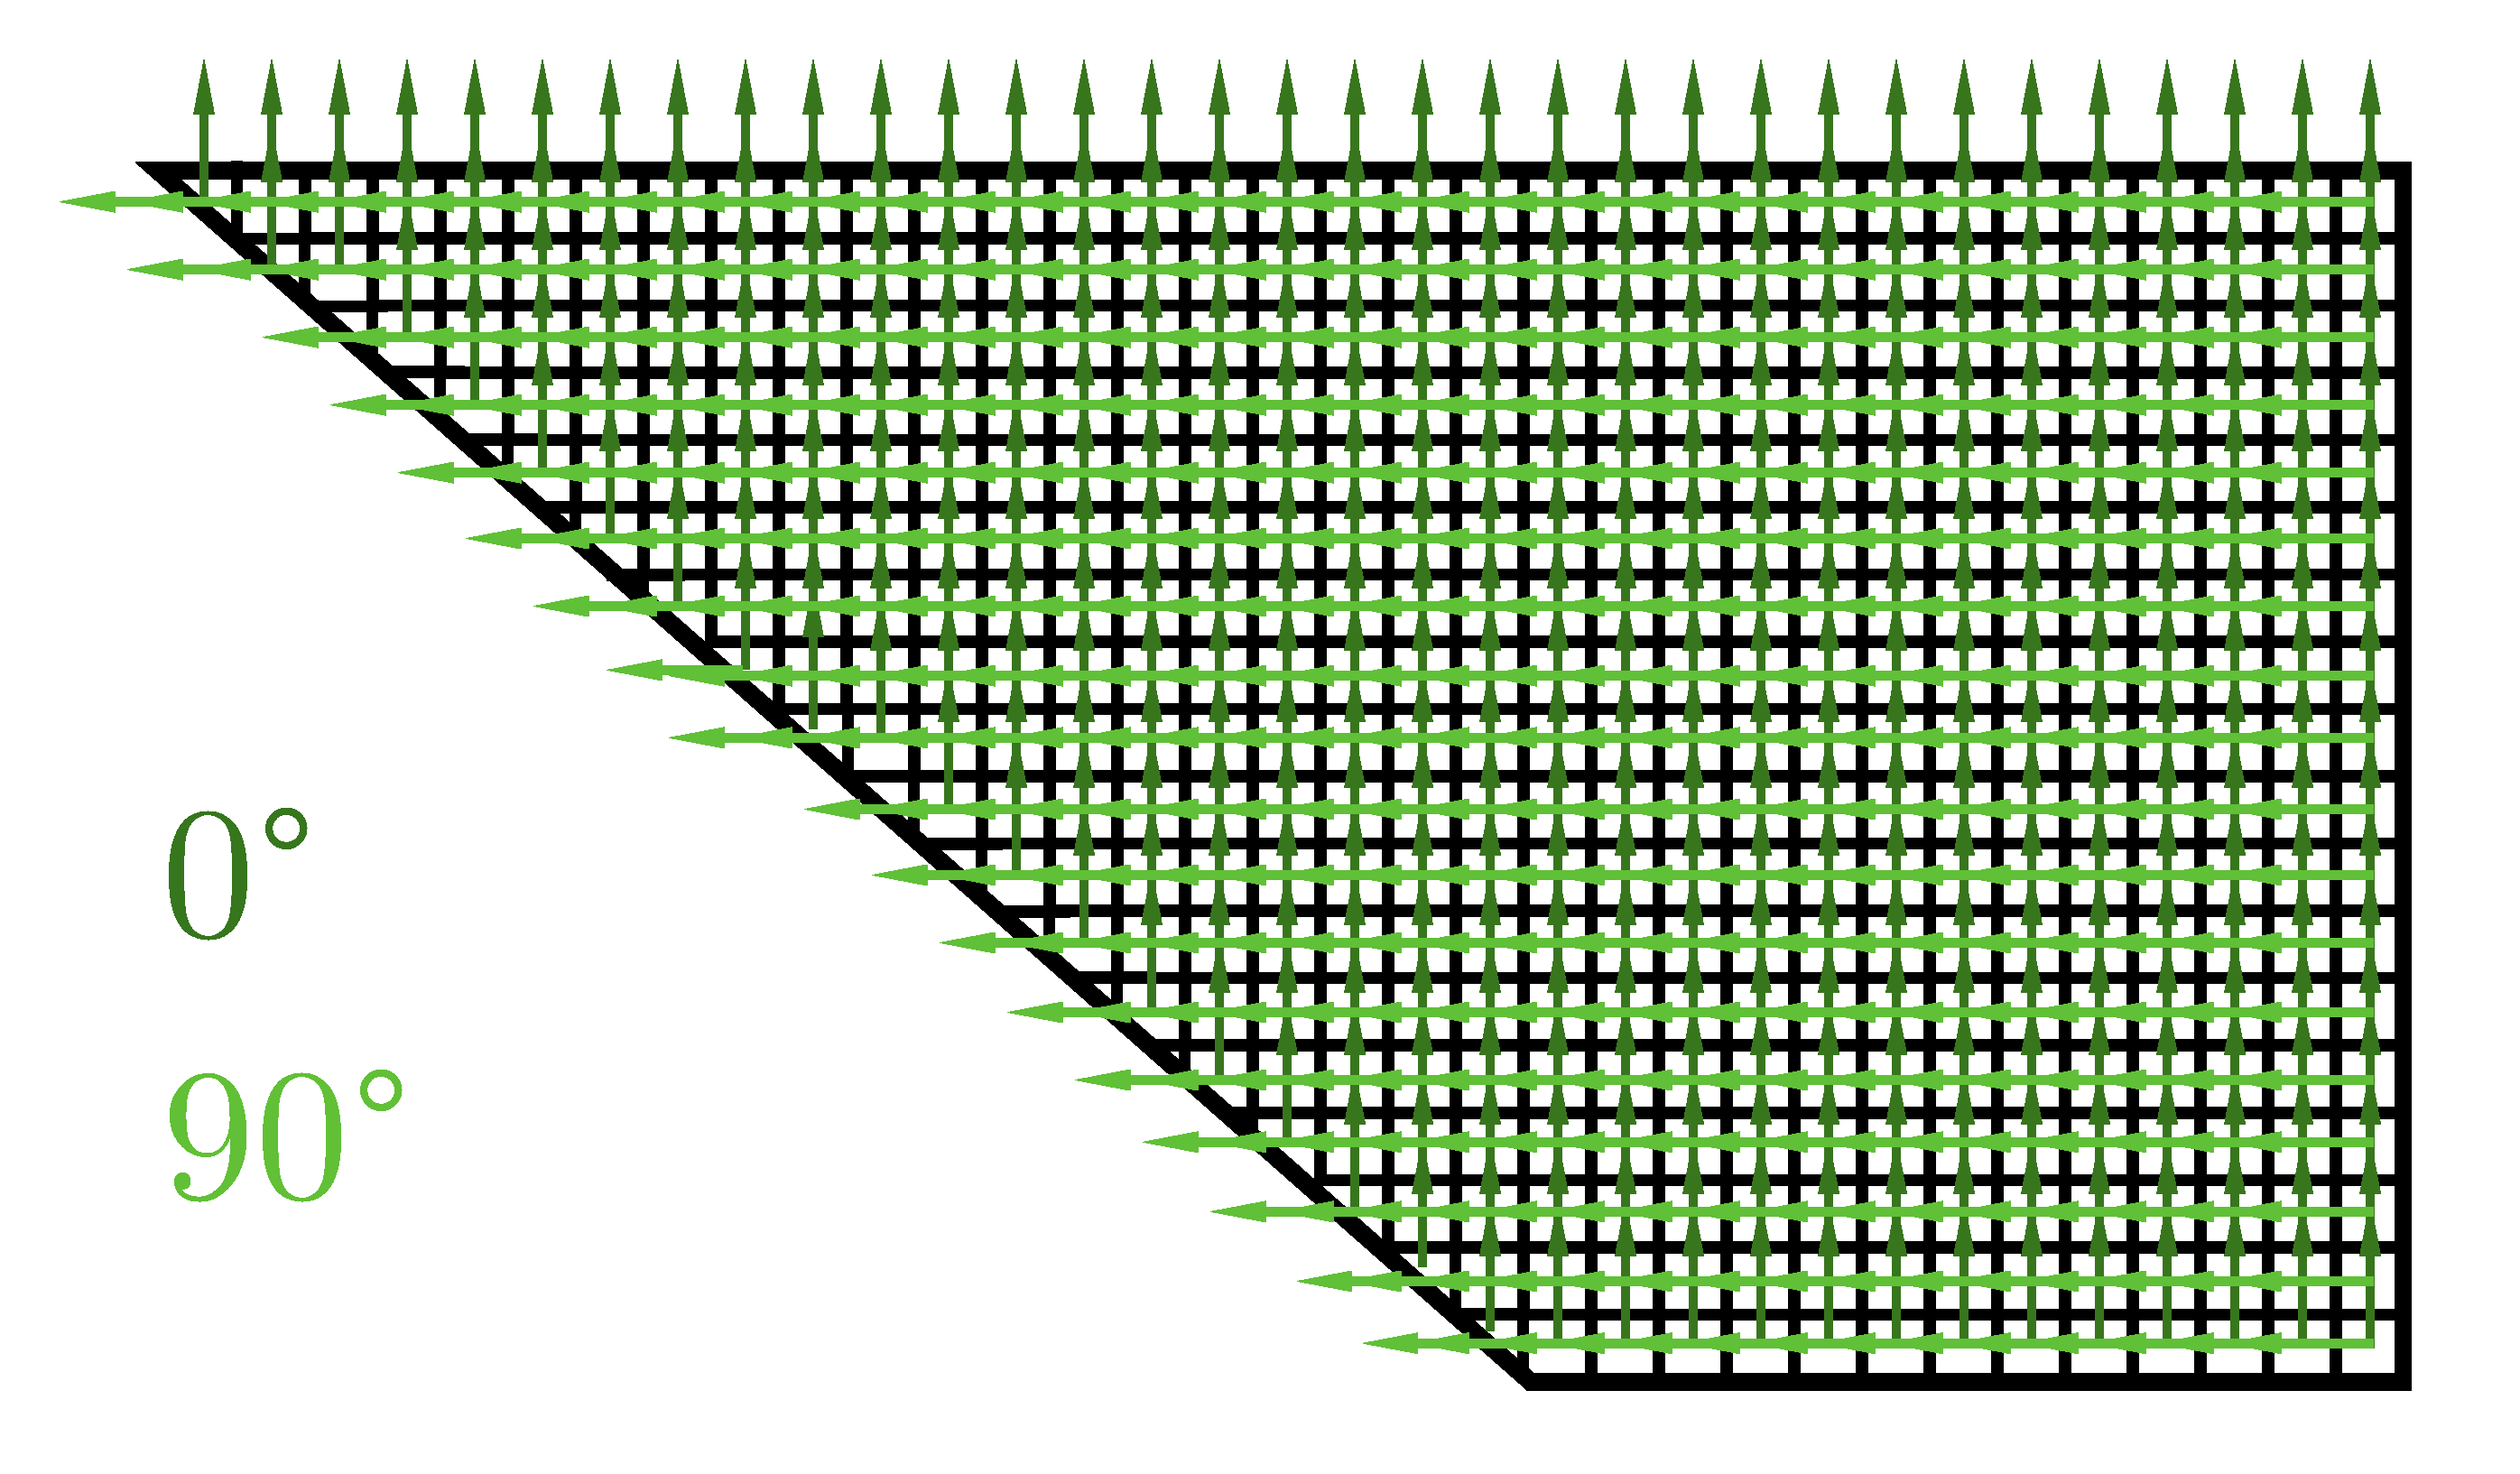
\includegraphics[scale=0.17]{0p90.pdf}~~~~~~~~
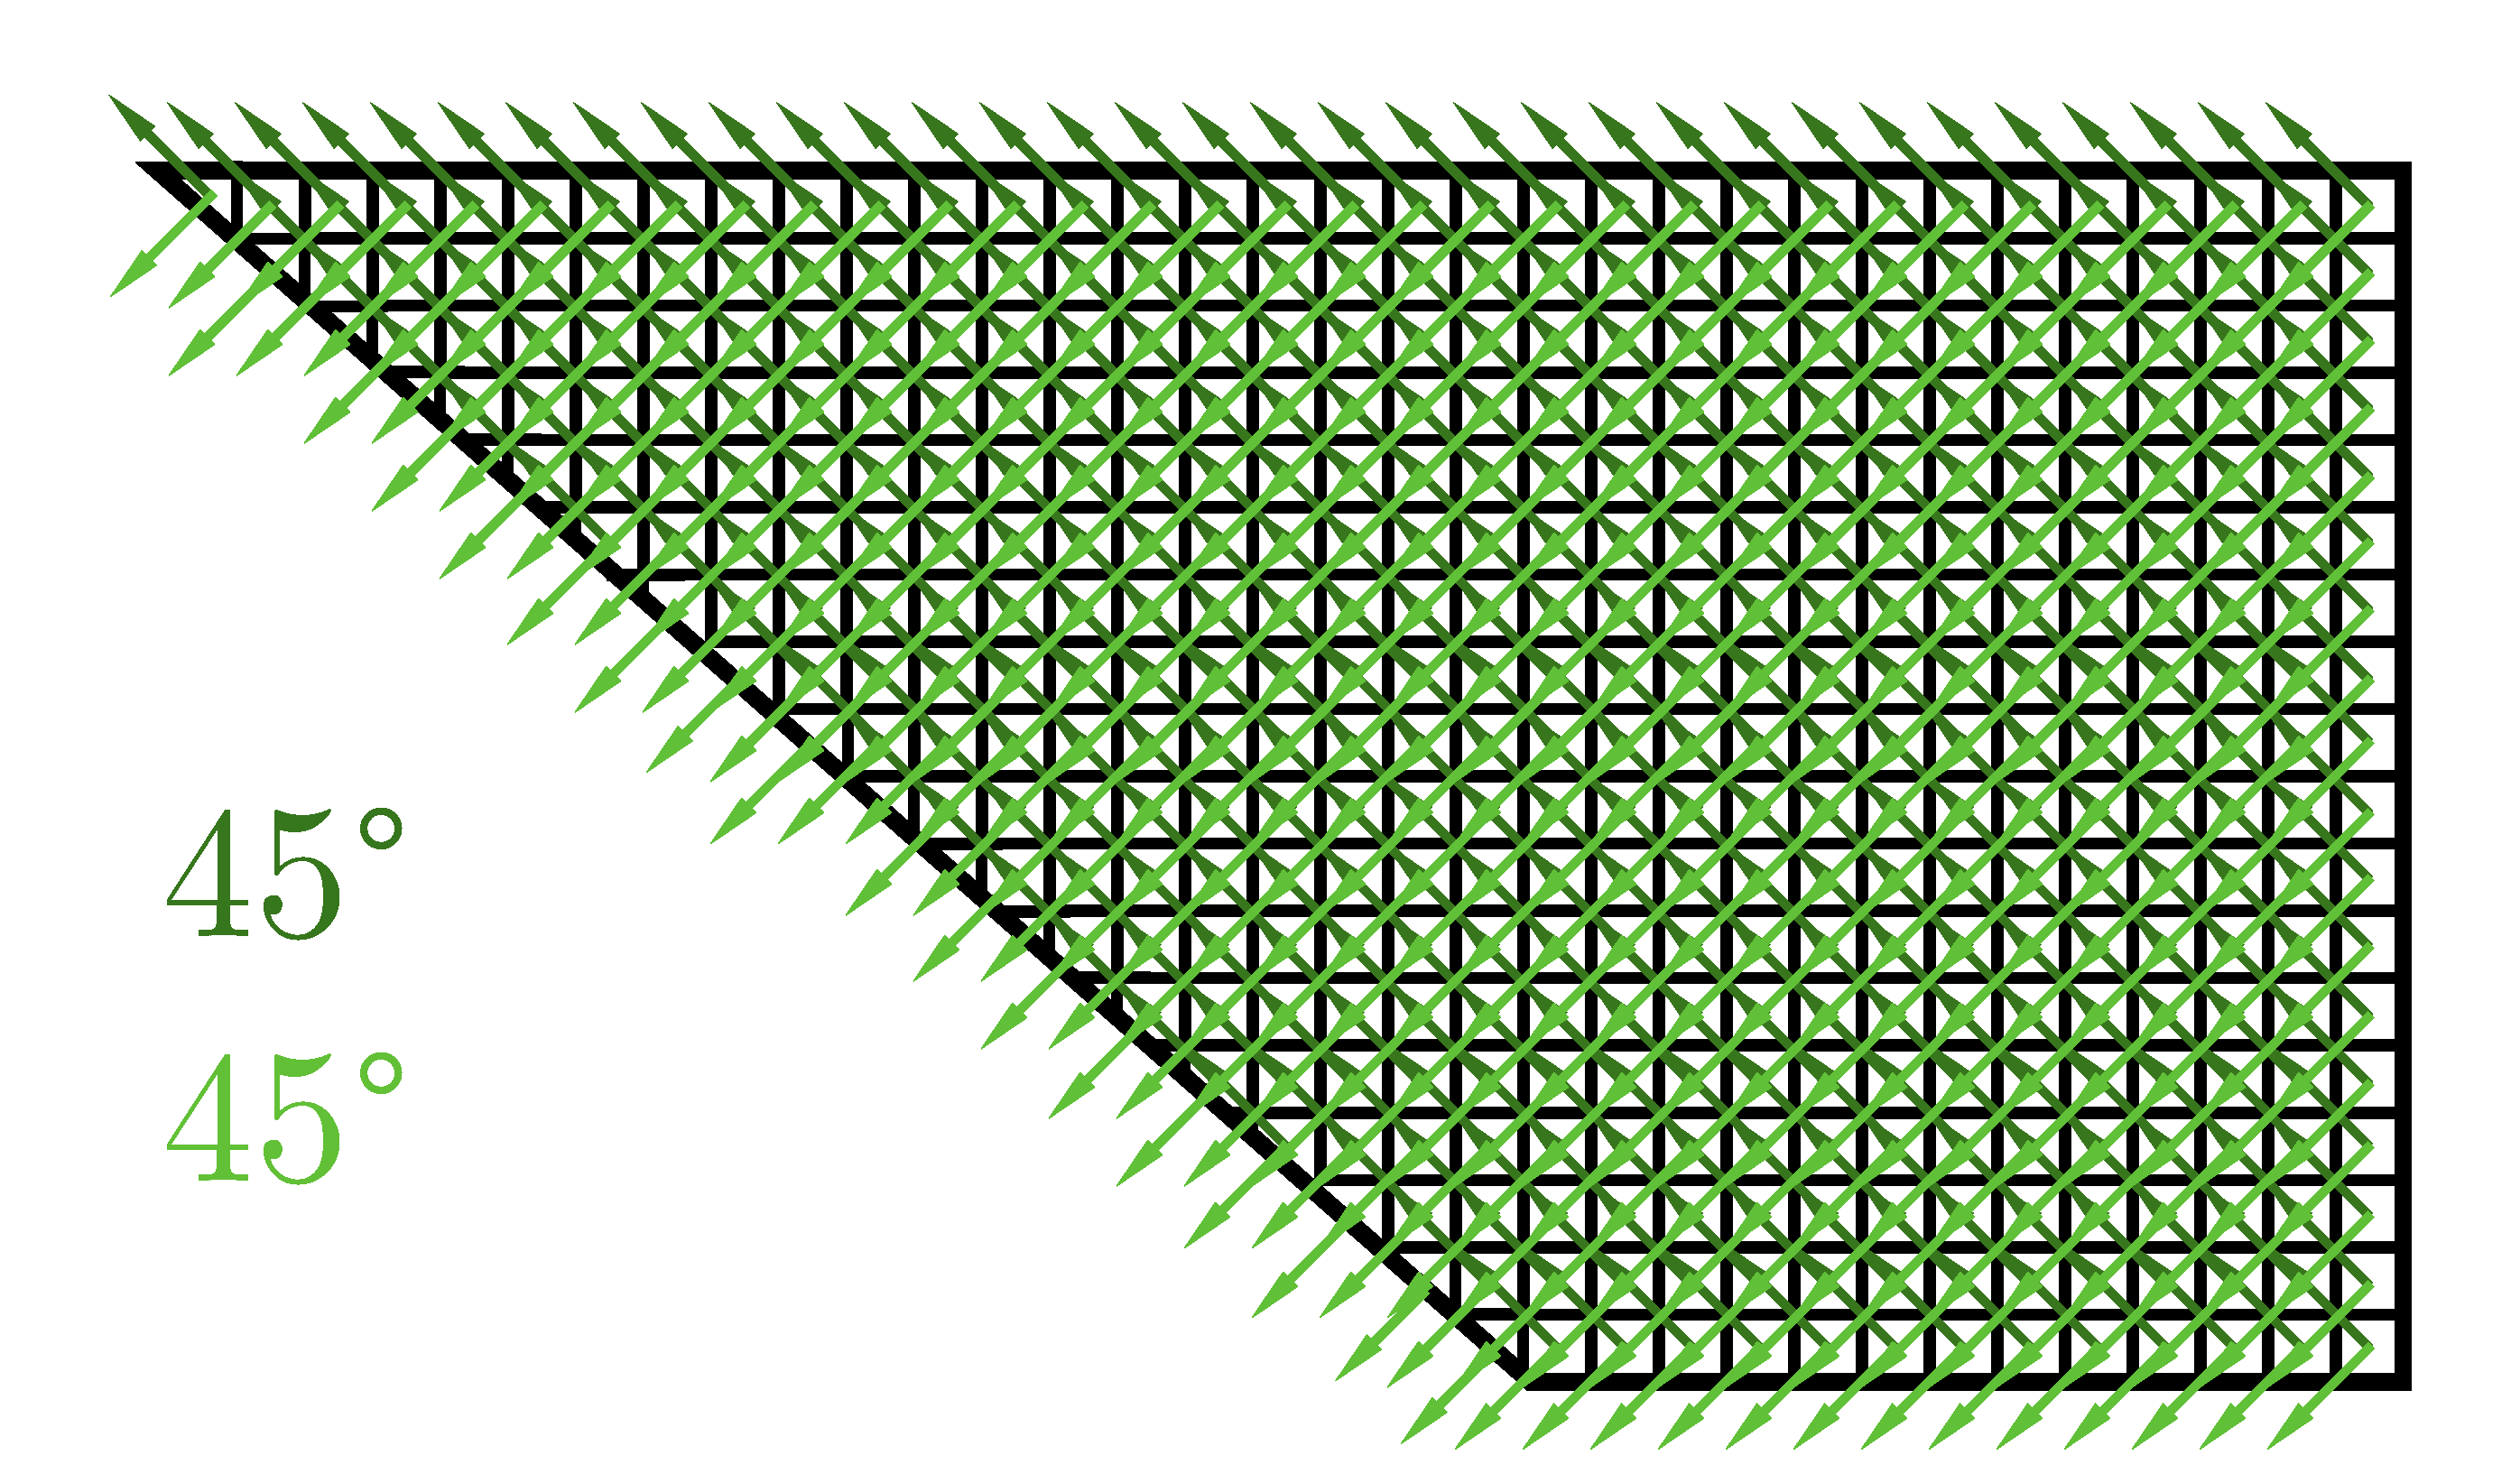
\includegraphics[scale=0.17]{45p45.pdf}
\caption{CF ply orientations: 0-90 and 45-45.}
\end{figure}
\noindent Once the CF 7-ply layup was complete, fillets were applied in order to smooth the leading, trailing, and outer edges; first, a 6$^\circ$ triangular cut was applied along the leading and outer edges, changing to 15$^\circ$ along the trailing edge. Then, fillet of radius 0.025" was applied along all edges. Technical drawings below illustrate this.
\begin{multicols}{2}
\begin{figure}[H]
\centering
\includegraphics[scale=0.02]{dessin2.pdf}	
\caption{Dimensions of fin before fillets.}
\end{figure}
\begin{figure}[H]
\centering
\includegraphics[scale=0.02]{dessin1.pdf}	
\caption{Dimensions of fin after fillets.}
\end{figure}

\end{multicols}
\begin{figure}[H]
\centering
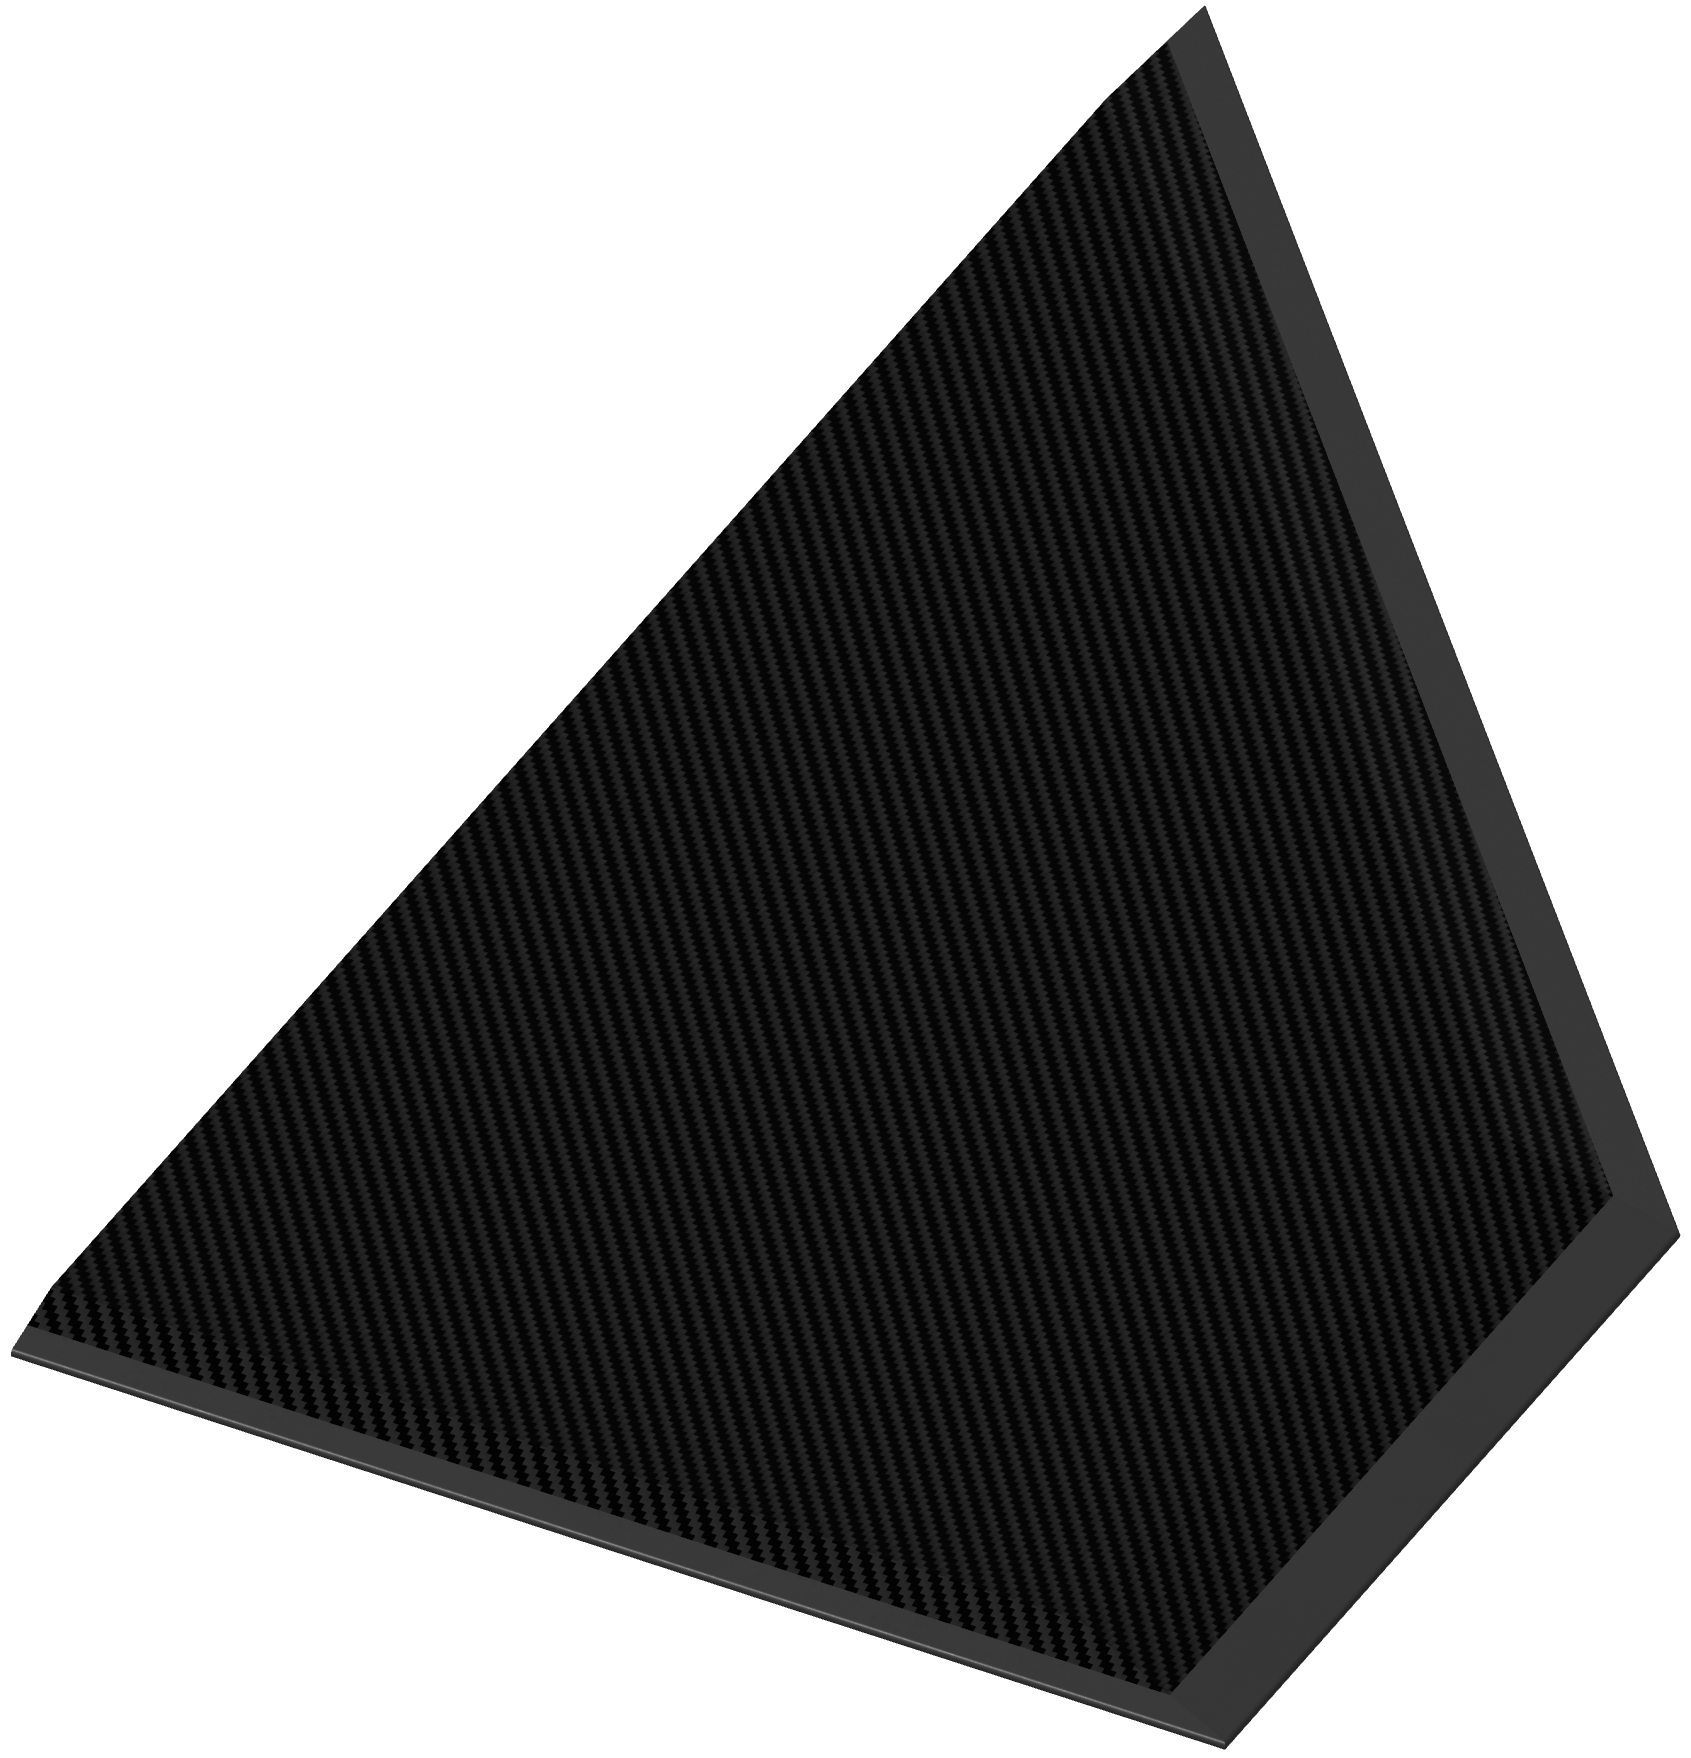
\includegraphics[scale=0.35]{render1.png}	
\caption{Render of a single fin, complete with layups and edge fillets.}
\end{figure}
~\\[1em]
\subsection{Simulation Process}
The process of simulation and determination of failure follows a few steps, starting from a blank project in Ansys Workbench.
\begin{multicols}{2}
\begin{enumerate}
	\item Use an \textbf{ACP Pre} block in ANSYS workbench.
	\item Define the material properties.
	\item Load Geometry using SpaceClaim.
	\item Mesh in \textit{Model}.
	\item Define Composite Layups, export as \textit{Solid}.
	\item Transfer model(s) to \textbf{Static Structure}.
	\item Define simulation parameters, then execute.
	\item Obtain composite failure and material deformation.
\end{enumerate}
\end{multicols}
\newpage
\subsection{Step 0: Obtain Relevant CAD Files}
In your preferred CAD (here SolidWorks is used), be sure to separate the objects of the CF plies and the G10 core, for a total of 3 objects. Export two STEP files: one with the G10 alone, and one with the CF alone. Name these in an unambiguous way.\\
\begin{figure}[H]
\centering
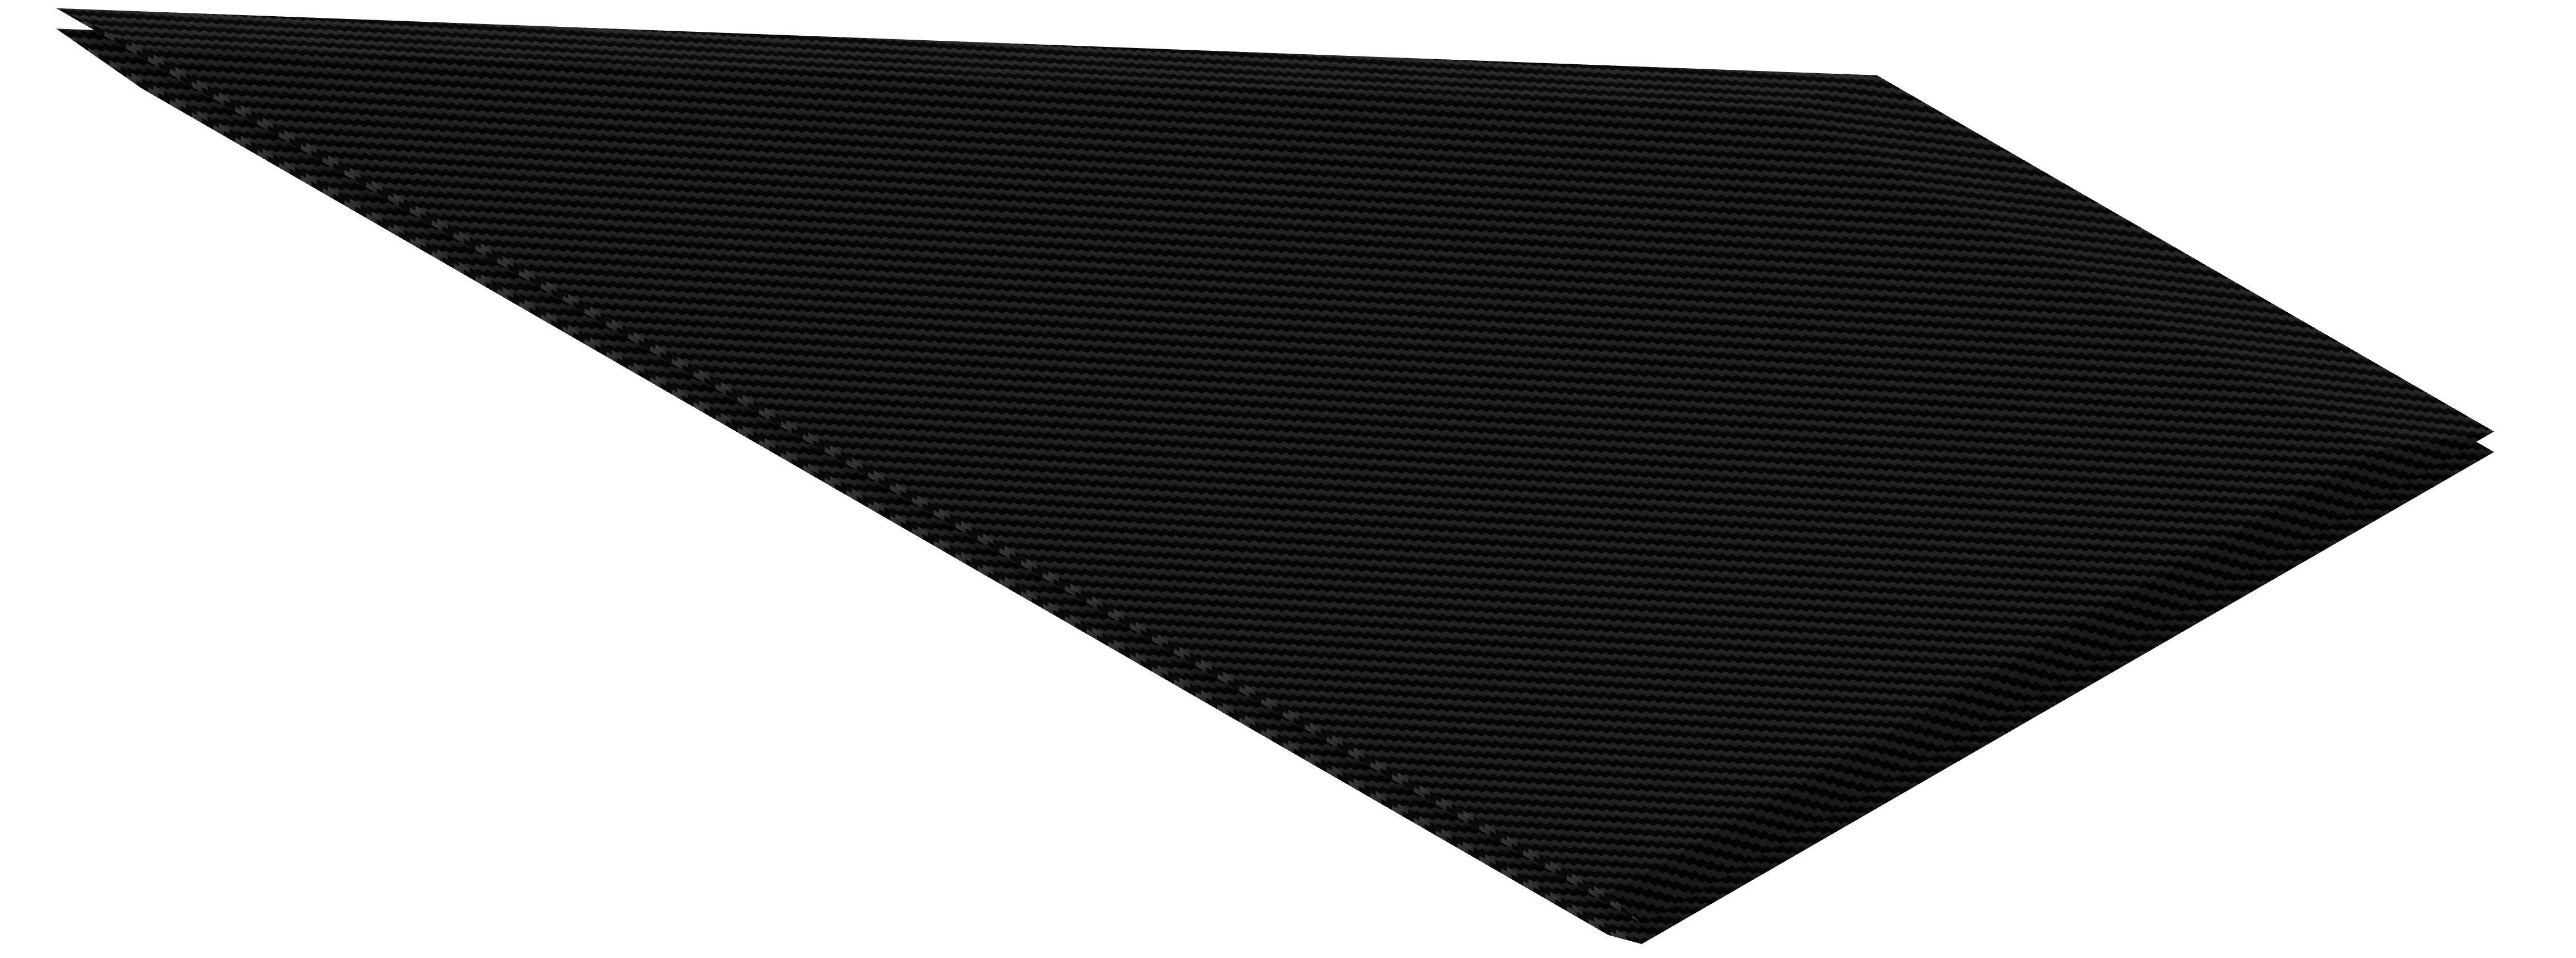
\includegraphics[scale=0.11]{CFonly.png}	\kern-1cm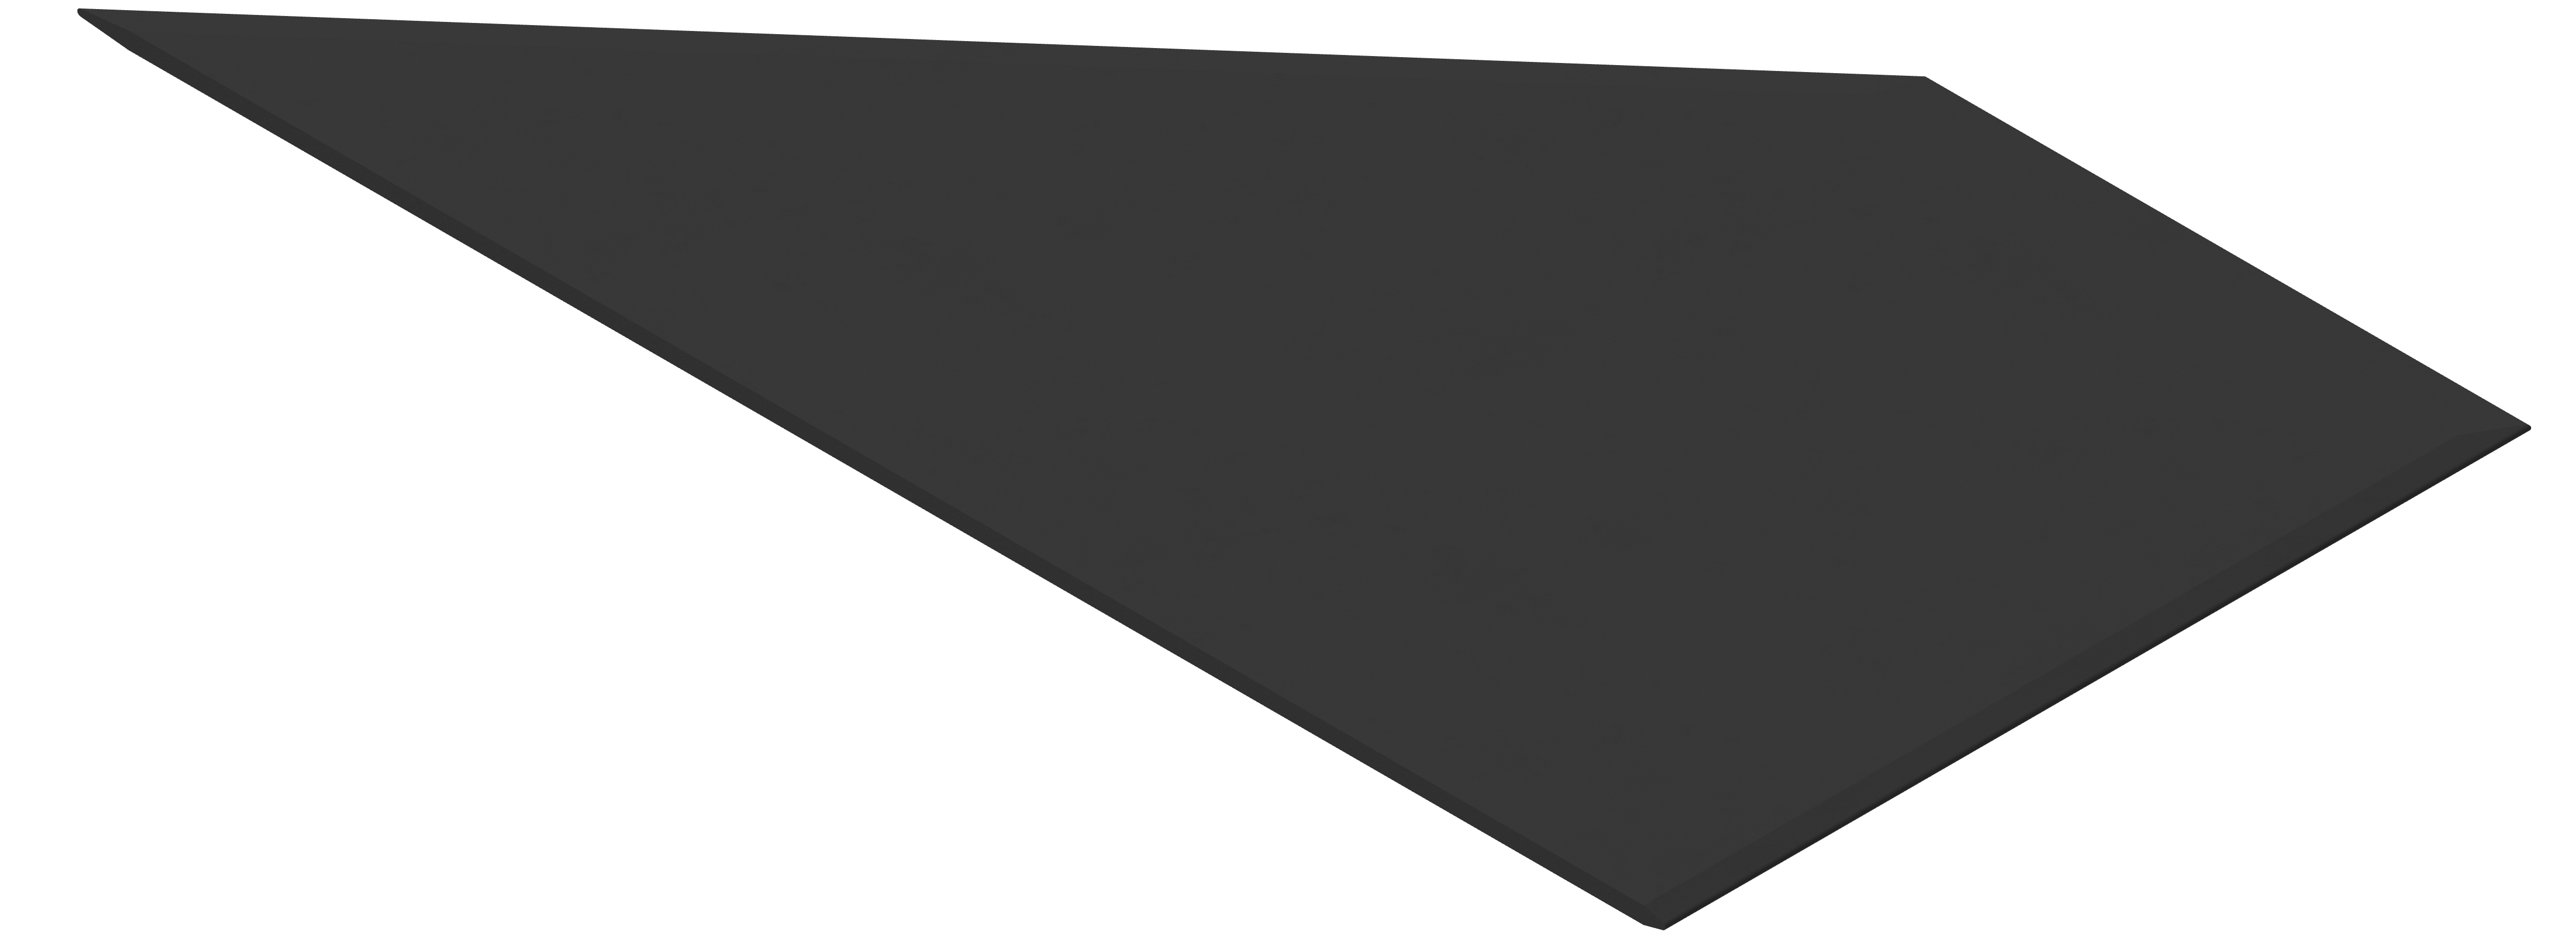
\includegraphics[scale=0.11]{G10only.png}	
\caption{Renders of CF Plies only (left) and G10 Core only (right).}
\end{figure}~\\
\noindent The G10 Core file will be used first; the CF Plies file will be used to trim the layups in the Composite definition step.\\

\subsubsection{Steps 1 and 2: Use an \underline{ACP Pre} method in ANSYS workbench; set the material properties.}~
\begin{multicols}{2}
	
\begin{figure}[H]
\centering
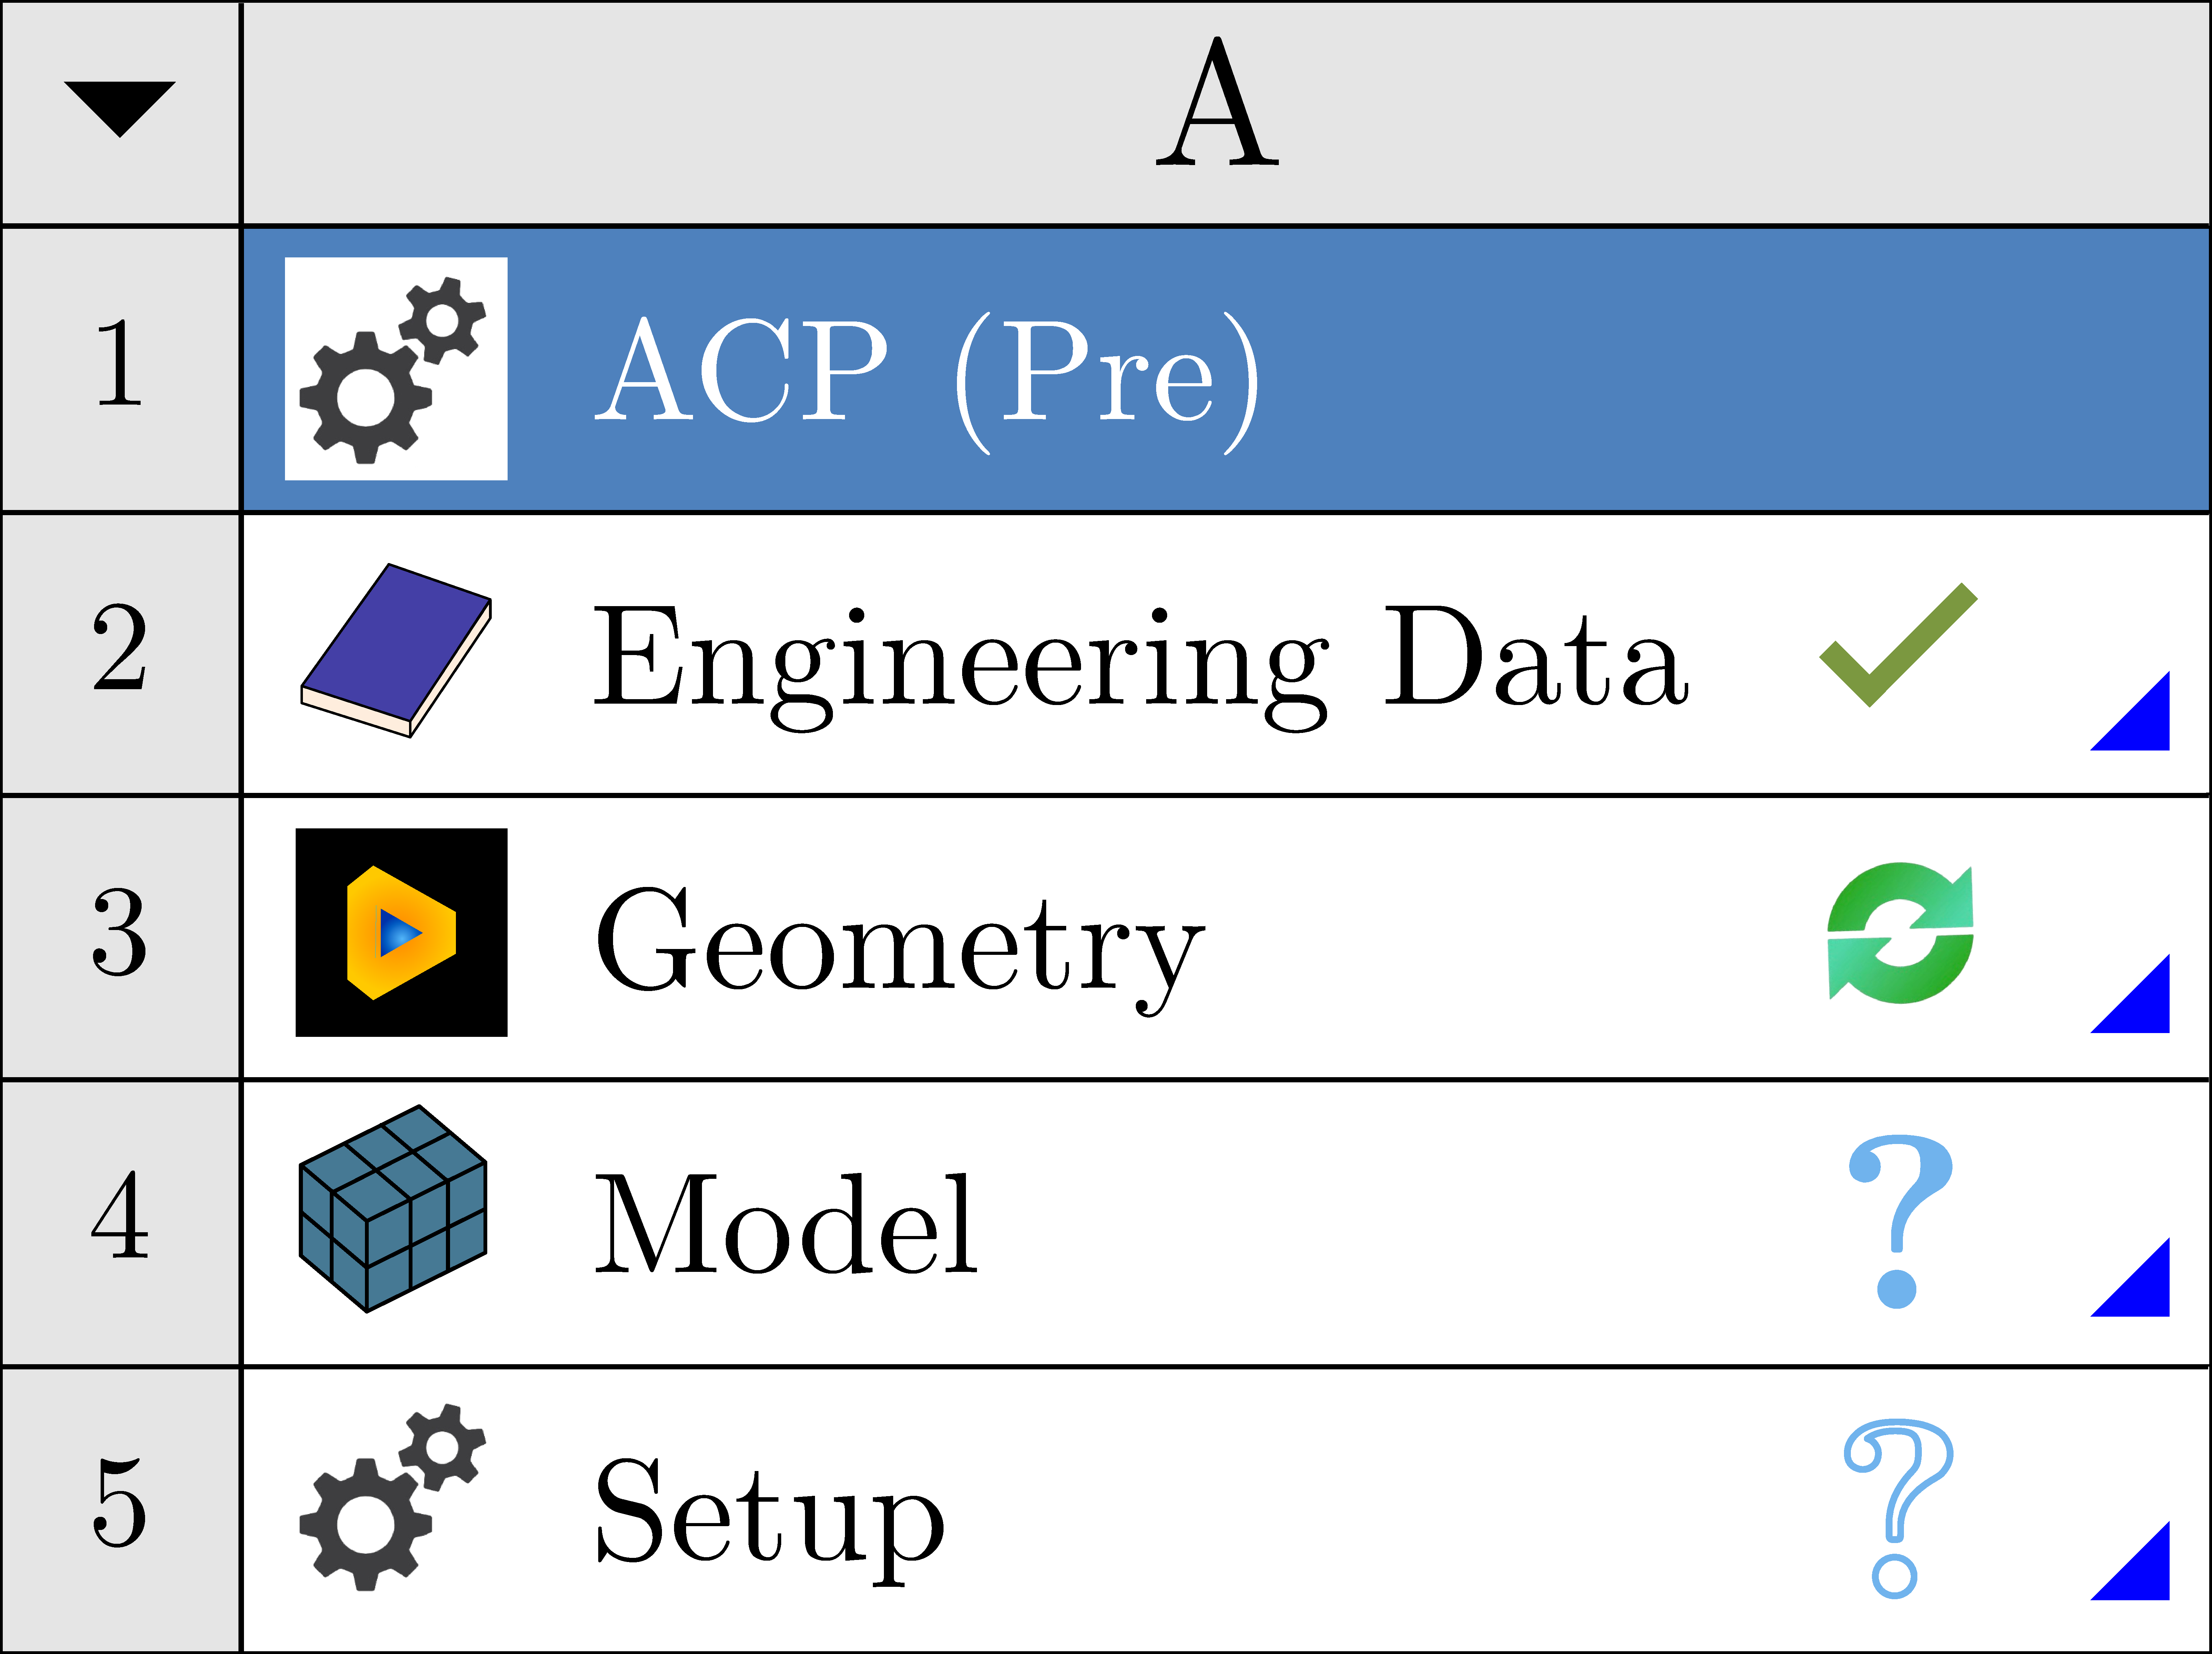
\includegraphics[scale=0.04]{ACPpre.pdf}	
\caption{An \textbf{ACP Pre} Block.}
\end{figure}
~\\\\We begin with the \textit{Engineering Data} block. Three materials were defined: the Carbon Fiber fabric, G10 plastic, and the Epoxy resin. Their properties are notedbelow. It is essential to enter these data correctly in order to obtain realistic simulation results.
\end{multicols}

\subsubsection{G10 Definition}
~\\[-3em]
\begin{table}[H]
\centering
\renewcommand{\arraystretch}{1.4}
~\kern-.4cm\begin{tabular}{l|c|c}
\bf Property & \bf Value & \bf Unit \\\hline\hline
Density & 2600 & kg m$^{-3}$ \\\hline
Coeff. of Therm. Exp. $\downarrow$ & & \\\hline
\quad Coeff. of Therm. Exp. & $5\cdot 10^{-6}$ & $^\circ$C$^{-1}$ \\\hline
Isotropic Elasticity $\downarrow$ & & \\\hline
\quad Derive from & Young \& Poisson & \\\hline
\end{tabular}~~~~~~
\begin{tabular}{l|c|c}
\bf Property & \bf Value & \bf Unit \\\hline\hline
\quad Young's Modulus & 18.6 & GPa \\\hline
\quad Poisson Coefficient & 0.27 & \\\hline
Thermal Conductivity & 1.27 & W m$^{-1}$ $^\circ$C$^{-1}$ \\\hline
Specific Heat Pressure & 802 & J kg$^{-1}$ $^\circ$C$^{-1}$\\\hline&&\\\hline
\end{tabular}
\end{table}

~
\subsubsection{Epoxy Resin (EPr) Definition}
~\\[-3em]
\begin{table}[H]
\centering
\renewcommand{\arraystretch}{1.4}
~\kern-.4cm\begin{tabular}{l|c|c}
\bf Property & \bf Value & \bf Unit \\\hline\hline
Density & 1160 & kg m$^{-3}$ \\\hline
Isotropic Elasticity $\downarrow$ & & \\\hline
\quad Derive from & Poisson \& Shear & \\\hline
\quad Young's Modulus & $5.4824\cdot 10^5$ & psi \\\hline
\end{tabular}~~~~~~
\begin{tabular}{l|c|c}
\bf Property & \bf Value & \bf Unit \\\hline\hline
\quad Shear Modulus & $2.0305\cdot 10^5$ & psi\\\hline
Elastic Tensile Limit & 7919.1 & psi \\\hline
Ply Type $\downarrow$ &  &\\\hline
\quad Type & Isotropic & \\\hline
\end{tabular}
\end{table}\newpage
\subsubsection{Carbon Fiber (CF) Definition}
~\\[-3em]

\begin{table}[H]
\centering
\renewcommand{\arraystretch}{1.4}
\begin{tabular}{l|c|c}
\bf Property & \bf Value & \bf Unit \\\hline\hline
Density & 1451 & kg m$^{-3}$ \\\hline
Orth. Coeff. of Therm. Exp.	$\downarrow$ & & \\\hline
\quad Coeff. of Therm. Exp. $\downarrow$ & & \\\hline
\quad \quad $X$ Coeff. of Ther. Exp. & $2.2\cdot10^{-6}$ & $^\circ$C$^{-1}$ \\\hline
\quad \quad $Y$ Coeff. of Ther. Exp. & $2.2\cdot10^{-6}$ & $^\circ$C$^{-1}$ \\\hline
\quad \quad $Z$ Coeff. of Ther. Exp. & $1.5\cdot10^{-5}$ & $^\circ$C$^{-1}$ \\\hline
Orth. Elasticity	$\downarrow$ & & \\\hline
\quad $X$ Young's Modulus & $5.916\cdot 10^{10}$ & Pa \\\hline
\quad $Y$ Young's Modulus & $5.916\cdot 10^{10}$ & Pa\\\hline
\quad $Z$ Young's Modulus & $7.5\cdot 10^{9}$ & Pa\\\hline
\quad Poisson Coeff: $XY$ & 0.04 & \\\hline
\quad Poisson Coeff: $YZ$ & 0.3 & \\\hline
\quad Poisson Coeff: $XZ$ & 0.3 & \\\hline
\quad Shear Modulus: $XY$ & $3.3\cdot 10^9$ & \\\hline
\quad Shear Modulus: $YZ$ & $2.7\cdot 10^9$ & \\\hline
\quad Shear Modulus: $XZ$ & $2.7\cdot 10^9$ & \\\hline
Orth. Stress Limits	$\downarrow$ & & \\\hline
\quad $X$ Tensile & $5.13\cdot 10^8$ & Pa\\\hline
\quad $Y$ Tensile & $5.13\cdot 10^8$ & Pa\\\hline
\quad $Z$ Tensile & $5\cdot 10^7$ & Pa\\\hline
\quad $X$ Compressive & $-4.37\cdot 10^8$ & Pa\\\hline

\end{tabular}~~~~~~
\begin{tabular}{l|c|c}
\bf Property & \bf Value & \bf Unit \\\hline\hline
\quad $Y$ Compressive & $-4.37\cdot 10^8$ & Pa\\\hline
\quad $Z$ Compressive & $-1.5\cdot 10^8$ & Pa\\\hline
\quad $XY$ Shear & $1.2\cdot 10^8$ & Pa\\\hline
\quad $YZ$ Shear & $5.5\cdot 10^7$ & Pa\\\hline
\quad $XZ$ Shear & $5.5\cdot 10^7$ & Pa\\\hline
Orth. Deformation Limits	$\downarrow$ & & \\\hline
\quad $X$ Tensile & $0.0092$ & \\\hline
\quad $Y$ Tensile & $0.0092$ & \\\hline
\quad $Z$ Tensile & $0.0078$ & \\\hline
\quad $X$ Compressive & $-0.0084$ & \\\hline
\quad $Y$ Compressive & $-0.0084$ & \\\hline
\quad $Z$ Compressive & $-0.011$ & \\\hline
\quad $XY$ Shear & $0.02$ & \\\hline
\quad $YZ$ Shear & $0.015$ & \\\hline
\quad $XZ$ Shear & $0.015$ & \\\hline
Tsai-Wu Constants $\downarrow$ & & \\\hline
\quad $XY$ Coupling & $-1$ & \\\hline
\quad $YZ$ Coupling & $-1$ & \\\hline
\quad $XZ$ Coupling & $-1$ & \\\hline
Ply Type $\downarrow$ & & \\\hline
\quad Type & Fabric\\\hline
\end{tabular}
\end{table}
~\\[-2em]
~\\\subsubsection{Step 3: Load Geometry Using SpaceClaim.}
Obtain the first STEP file, that with only the G10. Begin by right-clicking cell {\bf A3} in the ACP block, \textit{Geometry}, and choosing \textit{Import Geometry...} $\rightarrow$ \textit{Search}, and choose your first STEP file (substrate only, one body). Once the action is successfully completed, right-click the cell once more and choose \textit{Edit Geometry in SpaceClaim.} SpaceClaim will now launch. Once in SpaceClaim, the sidebar on the left will contain a model tree, resembling the following:
\begin{align*}
	&\downarrow ~\text{ACP-Pre} \\
	&\quad\rightarrow~\text{Body}
\end{align*}
In the main view, the STEP file will be displayed. In order to prepare the substrate for layup modeling, select the surfaces the CF will be bonded to (top and bottom faces), and copy-paste (\verb|ctrl-C, ctrl-V|). The model tree will now resemble the following:
\begin{align*}
	&\downarrow ~\text{ACP-Pre} \\
	&\quad\rightarrow~\text{Body}\\
	&\quad\rightarrow~\text{Surface}\\
	&\quad\rightarrow~\text{Surface}
\end{align*}
Name the surfaces according to their meaning: \verb|top| and \verb|bottom|, for example. Save your document (do not worry about path, ANSYS manages this for the user) by \verb|ctrl-S|, and close SpaceClaim.\\
\newpage
\subsubsection{Step 4: Mesh using Mechanical}
The next step is to right-click on cell {\bf A4} in the ACP block, \textit{Model}, and choose \textit{Edit}. In the tree on the left-hand side of the window that appears, search for the header of \textit{Geometry}:~\\[-3em]
\begin{multicols}{2}
	\begin{align*}
	&\downarrow ~\text{\bf Model (A4)} \\
	&\quad \rightarrow~{\color{Green}\checkmark}~\text{Geometry Import}\\
	&\quad \downarrow~{\color{red}\rm X}~\text{Geometry}\\
	&\quad \quad \rightarrow~{\color{red}\rm X}~\text{ACP-Pre$\backslash$Body}\\
	&\quad \quad \rightarrow~{\color{red}\rm X}~\text{ACP-Pre$\backslash$Surface}\\
	&\quad \quad \rightarrow~{\color{red}\rm X}~\text{ACP-Pre$\backslash$Surface}\\
	&\quad \rightarrow~{\color{Green}\checkmark}~\text{Materials}\\
	&\quad \rightarrow~{\color{Green}\checkmark}~\text{Coordinate System}\\
	&\quad \rightarrow~{\color{Green}\checkmark}~\text{Materials}\\
	&\quad \rightarrow~{\color{blue}\rm ?}~\text{Mesh}\\
	&\quad \rightarrow~{\color{Green}\checkmark}~\text{Named Selections}
\end{align*}
~\\[.5em]Choose the item \textit{ACP-Pre$\backslash$Body}, and in the lower window, choose the material associated with this body (G10) under the \textit{Materials} header of the info box in the lower right. For the two surfaces, associate the material and also specify a thickness $-$ as this is not physical, a small thickness $\left(10^{-10}\text{ m}\right)$ should be entered. Do not choose the object to be 2D, as this will prevent successful meshing and post processing.

Once the $\color{red} \rm X$s are gone and replaced with ${\color{Green}\checkmark}$s, proceed to the \textit{Mesh} item in the sidebar, and in the information box, choose under \textit{Size} to \textbf{\color{red} not} use an \textit{adaptive sizing}; input an element size of $\bf{0.00195}$ in the \textit{Element Size} box, just above the \textit{Size} header. 
\end{multicols}
When complete, click \textit{Generate} in the toolbar to generate the mesh. Depending on your hardware, this may take 10s of seconds to a minute. When complete, save using \verb|ctrl-S| and close Mechanical.

~\subsubsection{Step 5: Define Composite Layups, export as Solid.}
Right-click on cell \textbf{A5} in the ACP block, \textit{Setup}, and choose \textit{Edit}. In the window that appears, the sidebar on the left will contain a tree of properties and constructions relating to the composite. First, in the toolbar near the top of the window underneath the text \texttt{Scene.1}, click the \textit{generate} button, which has a lightning bolt symbol. Proceed to the sidebar; opening the submenus of \textit{Material Data} should generate a layout similar to the following:~\\[-3em]
\begin{multicols}{2}
\begin{align*}
	&\downarrow ~\text{\bf ACP-Pre} \\
	&\quad \downarrow~\text{Models} \\
	&\quad\quad \downarrow~\text{ACP Model} \\
	&\quad\quad\quad \rightarrow~\text{Scripts} \\
	&\quad\quad\quad \downarrow~\text{Material Data} \\
	&\quad\quad\quad\quad \downarrow~\text{Materials} \\
	&\quad\quad\quad\quad\quad \rightarrow~{\color{Green}\checkmark}~\text{G10} \\
	&\quad\quad\quad\quad\quad \rightarrow~{\color{Green}\checkmark}~\text{CF} \\
	&\quad\quad\quad\quad\quad \rightarrow~{\color{Green}\checkmark}~\text{EPr} \\	
	&\quad\quad\quad\quad \downarrow~\text{Fabrics} \\
	&\quad\quad\quad\quad \downarrow~\text{Stackups} \\
	&\quad\quad\quad\quad \downarrow~\text{Sub Laminates} \\
\end{align*}
~\\[.5em]
First, right-click \textit{Fabrics} and choose \textit{Create Fabric}. In the window that appears, choose the Material as \verb|CF| where the drop-down menu is colored {\color{red} red}. Specify the thickness as 0.009'' (SI Units: 0.00023 m). If desired, rename the fabric to a useful name, such as \verb|CFf|.

Next, right-click \textit{Stackups} and choose \textit{Create Stackup}. Name the stackup \verb|CFs|, if desired. A table of \textit{Fabric}s and \textit{Angle}s appears; this is where the stackup will be described. Fill out the table as follows:~\\[-2em]
\begin{table}[H]
\centering
\renewcommand{\arraystretch}{1.4}
\begin{tabular}{r|c|c|c|c|c|c|c|}
& 1 & 2 & 3 & 4 & 5 & 6 & 7\\\hline\hline
\bf Fabric & \tt CFf & \tt CFf & \tt CFf & \tt CFf & \tt CFf & \tt CFf & \tt CFf \\\hline
\bf Angle & \tt 0 &\tt 0 &\tt 45 &\tt 0 &\tt 45 &\tt 0 &\tt 0 \\\hline
\end{tabular}
\end{table}
~\\[-3em]
\end{multicols}
~\\[-3em]Move on to \textit{Element Sets}, opening the subfolder. Right-click on \verb|All_Elements| and choose \textit{Partition.} Two new element sets will appear, which should be renamed \verb|top| and \verb|bottom|, according to the reference frame chosen (it does not actually matter; by convention the force will be applied on the top face). 

Move on to \textit{Geometry}, and create a new \textit{CAD Geometry}. Choose the path of your \textbf{second} STEP file, the one with the CF plies only, and name the geometry \verb|adherence|. Choose \verb|Ok| to close the window and save the changes. Now, create a new \textit{Virtual Geometry}. Click in the \textit{sub shapes} box, then click on the \textit{CAD Geometry} you had just created. The text box should populate automatically; click \verb|Ok|.

Next, create the \textit{Rosettes}. Right-click \textit{Rosettes} and choose \textit{Create New}. Name it \verb|rTop|, and choose the corner where the trailing edge and root cord intersect on the \verb|top| element set. Choose the \verb|1| and \verb|2| directions such that the {\color{red} red} vector points along the trailing edge and the {\color{Green} green} vector points along the root chord. The {\color{blue} blue} vector will automatically point away from the fin core.
\begin{figure}[H]
\centering
\includegraphics[scale=0.04]{rosette.pdf}
\caption{Proper rosette orientation for a single fin.}	
\end{figure}
\noindent Perform the same operation for the \verb|bottom| element set; the {\color{blue} blue} vector will still automatically point away from the fin core.

Next, create an \textit{Oriented Selection Set}.




\end{document}